\documentclass[nostrict]{szablonPG}

\usepackage{listing_schemat}

\begin{document}

%\includepdf{meta/strona_tytulowa.pdf}
%\includepdf{meta/oswiadczenie.pdf}

\chapter*{Streszczenie}
\textbf{Słowa kluczowe:} 

\textbf{Dziedzina nauki i techniki, zgodnie z wymogami OECD:} 

\chapter*{Abstract}


\noindent\textbf{Keywords:} 


\tableofcontents

\chapter*{Wykaz ważniejszych oznaczeń i skrótów}
\begin{labeling}[align=right,labelwidth=5cm]
    \item [LZWP, Laboratorium] Laboratorium Zanurzonej Wizualizacji Przestrzennej, znajdujące się w budynku A wydziału ETI Politechniki Gdańskiej.
    \item [Duża Jaskinia] główna jaskinia rzeczywistości wirtualnej, składająca się z sześciu ścian.
    \item [Średnia Jaskinia] jaskinia rzeczywistości wirtualnej składająca się z czterech ścian - prawej, lewej, frontalnej oraz dolnej.
    \item [Mała Jaskinia] środowisko stworzone z czterech monitorów, pomniejszona wersja średniej jaskini.
\end{labeling}


\chapter{Opis i cel projektu}

\newcommand{\chapterPath}{rozdzialy/1_opis}

\section{Inspiracja}
W 2003 roku niejaki Barrett Lyon, informatyk oraz artysta, postawił sobie za cel stworzenie wiernego odwzorowania połączeń między komputerami w sieci Internet. Wizualizacja grafu miała być zrealizowana za pomocą kolorowych linii oraz punktów. W ten sposób, w październiku 2003 roku powstał open source-owy Projekt Opte. Głównym celem tego projektu było zilustrowanie wciąż szybko rozwijającego się Internetu oraz wyróżnienie regionów, które w tamtych czasach doświadczały gwałtowny wzrost łączności z Internetem.
Projekt szybko zyskał dużą popularność, a jeden z efektów końcowych można było zobaczyć na żywo w Muzeum Sztuki Nowoczesnej w Nowym Jorku. Przykładową wizualizację zaprezentowano na Rysunku 1. Twórca Opte Project w artykule dla Time[1] krótko podsumował swoją motywację:
The Internet is really big, very connected and extremely complex.
It’s this whole world you can’t see. That’s the fun part of visualizing it.

\section{Opis projektu}
Tak jak w przypadku Opte Project, głównym zadaniem projektu jest przygotowanie grafu oraz jego wizualizacja. Nie jest to jednak graf połączeń sieci Internet, lecz sieć artykułów i kategorii internetowej encyklopedii Wikipedia. Tworzona jest ona na podstawie odnośników znajdujących się w treści artykułu, prowadzących do innych, tematycznie powiązanych, artykułów.

Nasza aplikacja oferuje nowy i innowacyjny sposób na przeglądanie Wikipedii: poprzez wizualizację połączeń pomiędzy artykułami. Dostępne są również narzędzia pozwalające na sprawne poruszanie się po grafie jak i dodatkowe funkcjonalności służące podstawowej analizie prezentowanych danych.

W celu pogłębienia immersji aplikacja została napisana na środowisko jaskini zanurzonej rzeczywistości wirtualnej znajdującej się w LZWP (Laboratorium Zanurzonej Wizualizacji Przestrzennej). Mając do dyspozycji widok ze wszystkich stron można przenieść użytkownika w dowolne miejsce skomplikowanego grafu co pozwoli mu przyjrzeć się połączeniom z bliska i lepiej zrozumieć strukturę Wikipedii.

\section{Główne cele projektu}
Głównym celem projektu jest propozycja rozwiązania mającego zainteresować oraz inspirować odbiorców nietypowym przedstawieniem znanej powszechnie Wikipedii. Nietypowość polega głównie na~zmianie medium, przez które użytkownicy zwykle odbierają Wikipedię. Zamiast traktować ją jako zbiór artykułów, skupiamy się na uwidocznieniu związków między nimi, które mogłyby być trudne do~uchwycenia podczas przeglądania stron encyklopedii w przeglądarce internetowej.

Aplikacja wzbogaci nieustannie powiększający się zestaw materiałów dydaktycznych przygotowywanych w środowisku Laboratorium Zanurzonej Wizualizacji Przestrzennej na Politechnice Gdańskiej. Różnorodne aplikacje pozwalają lepiej zaprezentować możliwości rozwiązań wizualizacji przestrzennej gościom odwiedzającym LZWP.
\section{Interesariusze i użytkownicy}
Projekt jest realizowany jako projekt inżynierski pod opieką dr inż. Jacka Lebiedzia. Jest on głównym interesariuszem, a także jednym z użytkowników. Pozostałymi użytkownikami są osoby pracujące w laboratorium, goście zaproszeni w celu prezentacji jego możliwości i oprogramowania oraz zespół deweloperski opracowujący aplikację. Szczegółowa lista interesariuszy i użytkowników zamieszczona została w tablicy \ref{tab:users-stakeholders}.
\\
\tabela{
	\hline
	\textbf{Interesariusz/użytkownik} & \multicolumn{1}{ c| }{\textbf{Opis}} \\\hline
	dr inż. Jacek Lebiedź & Opiekun projektu inżynierskiego oraz kierownik LZWP, wykładowca na WETI PG, pracownik Katedry Inteligentnych Systemów Interaktywnych \\\hline
	Pracownicy laboratorium & Zespół pracowników laboratorium rozwijający oprogramowanie jaskini oraz oferujący pomoc w dostosowaniu aplikacji do środowiska i warunków LZWP \\\hline
	Zespół deweloperski & Osoby pracujące nad aplikacją \\\hline
	Goście LZWP & Zaproszone osoby, którym prezentowane są możliwości jaskini na różnego rodzaju wydarzeniach, m.in. konferencjach i dniach otwartych \\\hline
}{ |c|p{0.6\textwidth}| }{Zestawienie interesariuszy i użytkowników projektu}{users-stakeholders}


\begin{chapter}{Specyfikacja wymagań projektu}
	\newcommand{\chapterPath}{rozdzialy/2_wymagania}
	
	Ten rozdział obejmuje opis wymagań funkcjonalnych, jakościowych oraz technicznych projektu, a także kilka przypadków użycia. Był przygotowywany przed rozpoczęciem prac nad aplikacją i zostanie zwalidowany i skomentowany w podsumowaniu pracy.

	\section{Wymagania funkcjonalne}
Budowa aplikacji musi być zgodna z wymaganiami jaskini rzeczywistości wirtualnej. Aplikacja będzie uruchamiać się jednocześnie na wielu komputerach, dlatego dane muszą się aktualizować dostatecznie szybko, aby zachować płynność i zgodność wyświetlanych obrazów.

Aplikacja musi posiadać kilka widoków przeglądania danych: widok grafu, widok szczegółowy oraz widok węzła, który dzieli się na widok artykułu i widok kategorii.

Widok grafu (Rysunek \ref{fig:prototyp_widok_grafu}) jest głównym widokiem aplikacji. Użytkownik może się w nim swobodnie poruszać (``latać'') we wszystkich kierunkach. Widoczne są artykuły i kategorie umieszczone w przestrzeni w formie ``punktów''. Obiekty są ze sobą ściśle powiązane, tworzą strukturę grafu (możliwe są jednak węzły nie posiadające żadnych połączeń). Same połączenia w widoku nie są wyświetlane w celu zachowania przejrzystości wyświetlanych informacji. Artykuły i kategorie można wskazywać, a następnie wybierać. Po wykonaniu tej czynności przechodzimy do widoku artykułu lub widoku kategorii - w zależności od typu wybranego węzła. Oba te widoki nazywamy w ogólności widokiem węzła.

\img{\chapterPath/img/prototyp_widok_grafu.jpg}{Prototyp widoku grafu}{prototyp_widok_grafu}{0.8}

Widok węzła przedstawia wybrany węzeł na dolnym ekranie oraz połączenia z innymi węzłami. Aby ułatwić wskazywanie połączeń, połączone węzły będą pokazywane w formie otaczających użytkownika kopii ``punktów'' i będą zawieszone na krzywych biegnących od wybranego węzła z dolnego ekranu do oryginalnego ``punktów''. W zależności od tego, czy wybrany jest artykuł czy kategoria, mamy dwa tryby wyświetlania powiązań. Jeśli wybraliśmy artykuł, w pierwszym trybie wyświetlane są powiązane artykuły (w sensie wystąpienia linku do tego artykułu w wybranym artykule), a w drugim najniższe (najbardziej szczegółowe) kategorie, do których należy wybrany artykuł. Pierwszy tryb został zilustrownay na Rysunku \ref{fig:prototyp_widok_wezla}.

\img{\chapterPath/img/prototyp_widok_wezla.jpg}{Prototyp widoku węzła (przypadek widoku powiązań artykułów)}{prototyp_widok_wezla}{0.8}

W przypadku wybrania kategorii wyświetlane są albo artykuły i kategorie, które bezpośrednio należą do wybranej kategorii, albo najniższe kategorie, do których należy wybrana kategoria. Aby nie przytłaczać użytkownika zbyt dużą ilością informacji, wyświetlana jednocześnie liczba połączeń jest ograniczona, utworzone przedziały będzie można przewijać. Po wybraniu połączonego węzła przenosimy się do widoku nowo wybranego węzła. Możliwe jest cofanie się w historii przeglądania, a także ponowne wykonywanie cofniętej operacji. W tle widoczne są węzły z widoku grafu, jednak wyłączona jest możliwość ich wybierania w celu ułatwienia wskazywania powiązań. Nazwa wybranego węzła wyświetlana jest na górze i zmienia swoją pozycję poziomą, śledząc ruch głowy użytkownika. Istnieje opcja automatycznego poruszania się po powiązaniach artykułów i kategorii, która ułatwia prezentację aplikacji. Polega ona na przechodzeniu do losowo wybranych węzłów powiązanych z aktualnie wybranym do momentu, w którym zostanie ona ręcznie zatrzymana. W każdym momencie możliwe jest opuszczenie widoku węzła i przejście do widoku grafu. Zostajemy wtedy ustawieni obok węzła, z którego widoku wyszliśmy. Z każdego widoku jest możliwe także przejście do widoku grafu z kamerą wycentrowaną na główną kategorię całego grafu. Do widoku szczegółowego można przejść z poziomu widoku węzła. Wyświetlane są w nim statystyki dotyczące węzła i informacje ogólne na temat strony.

W trybie grafu i trybie węzła na górnej części widoku widoczna jest także oś czasu. Pokazuje ona czas, z którego wyświetlany jest stan grafu i wybraną jednostkę czasu. Zmienia ona swoje położenie na podstawie ruchów głowy użytkownika tak, aby zawsze znajdowała się nad nim. Zmiana czasu na osi powoduje pokazywanie tylko takich węzłów, które istniały w wybranym czasie (wraz z ich połączeniami).

Aplikacja wymaga zastosowania dwóch kontrolerów ze względu na dużą liczbę interakcji dostępną dla użytkownika. Aby zapewnić wyższą jakość obsługi zaimplementowana zostanie opcja wyboru układu przycisków - praworęczny oraz leworęczny. Wybór ten będzie możliwy przy starcie aplikacji. W momencie wyświetlania okna wyboru widoczna będzie także infografika z informacjami o sterowaniu. Będzie można  otworzyć ją także w trakcie przeglądania danych. Z pozycji infografiki można także zmienić tryb sterowania za pomocą wyświetlanego przycisku.

Za pomocą głównego kontrolera (Rysunek \ref{fig:schemat_kontroler_glowny}) będzie można wskazywać i wybierać węzły zarówno w widoku grafu, jak i w widoku węzła. Za pomocą joysticka w każdym widoku można dokonywać ruchu kamerą. W widoku grafu służy on także do swobodnego poruszania się, a w widoku węzła do przesuwania grup połączeń. Cztery pozostałe przyciski służą do resetowania widoku do stanu początkowego (przycisk Home), cofania się w historii przeglądania (przycisk Back), ponowienia cofniętej historii przeglądania (przycisk Forward) oraz opuszczenia widoku węzła i przejście do widoku grafu (przycisk Exit).

\img{\chapterPath/img/schemat_kontroler_glowny.png}{Schemat kontrolera głównego}{schemat_kontroler_glowny}{0.8}

Kontroler pomocniczy (Rysunek \ref{fig:schemat_kontroler_pomocniczy}) wykorzystuje joystick oraz trzy przyciski. Joystick służy do manipulowania osią czasu. Za jego pomocą można zmieniać jednostkę czasu oraz dokonywać zmiany czasu. Pierwszy przycisk służy do automatycznej wycieczki po węzłach (przycisk Auto, ponowne jego naciśnięcie zatrzymuje wycieczkę) oraz do wyświetlenia szczegółów i statystyk wybranego artykułu (przycisk Details). Oba przyciski dostępne są tylko w trybie widoku węzła. Trzeci przycisk (przycisk Help) powoduje wyświetlenie pomocy z infografiką o sterowaniu, która jest dostępna w każdym widoku.

\img{\chapterPath/img/schemat_kontroler_pomocniczy.png}{Schemat kontrolera pomocniczego}{schemat_kontroler_pomocniczy}{0.8}

	\section{Wymagania jakościowe}
\begin{enumerate}[label=\textbullet]
\item \textbf{Niezawodność}

Aplikacja nie może posiadać żadnych błędów, które powodowałyby zaburzenie immersji. Należą do nich wszelkie błędy graficzne, błędy w interfejsie, jak również nieprawidłowe umiejscowienie węzłów i połączeń w przestrzeni. Aplikacja musi mieć także dobrze zaprojektowaną i przemyślaną strukturę grafu, ponieważ stanowi ona rdzeń programu. Jakiekolwiek błędy z nią związane powodowałyby niezdolność do korzystania z aplikacji i niepowodzenie całego projektu. W przypadku wykrycia takich błędów powinny one uzyskać najwyższy priorytet i być naprawione w następnej wersji.

\item \textbf{Użyteczność}

Aplikacja musi być estetyczna i wygodna w użyciu. Ważne jest zastosowanie nowoczesnych animacji i innowacyjnego interfejsu, pozwalającego zanurzyć się w wizualizacji. Użytkownik ma się poczuć, jakby naprawdę podróżował po stworzonym świecie. Interfejs musi wykorzystywać zalety jaskini rzeczywistości wirtualnej - możliwość ruchu użytkownika i śledzenie ruchów głowy. Aby zapewnić widok dla wielu osób maksymalnie niezależny od pozycji okularów wiodących obiekty muszą znajdować się w odległości odpowiadającej pozycji ścian jaskini. Sterowanie aplikacją, mimo dużej ilości interakcji, powinno być intuicyjne, a w razie problemów musi istnieć pomoc dla użytkownika.

\item \textbf{Czas reakcji}

Aplikacja, ze względu na swoją specyfikę, musi być przyjemna w odbiorze dla użytkownika. Czas przejścia z widoku grafu do widoku węzła lub odwrotnie oraz czas podróży pomiędzy węzłami nie powinien trwać więcej niż 1,5 sekundy. Dopuszczalny jest długi czas uruchamiania aplikacji ze względu na wymóg zbudowania grafu z pliku, jednak nie powinien on trwać więcej niż 20 sekund, gdyż spowodowałoby to obniżenie zadowolenia użytkownika i spowolniłoby to prezentowanie możliwości jaskini odwiedzającym. 
\end{enumerate}
	\section{Wymagania techniczne}
Aby projekt został zaliczony, kluczowe jest jego poprawne działanie w środowisku jaskini rozszerzonej rzeczywistości wirtualnej. Na komputerach obsługujących jaskinię działa aktualnie system Windows 7. Aplikacje wykorzystujące jaskinię zbudowane są w oparciu o środowisko Unity. Użycie najnowszych wersji platformy nie jest zalecane z powodu braku kompatybilności. Z tego powodu projekt jest realizowany w Unity 2018.1.9 oraz używa platformy .NET 4.x.

Do działania aplikacji są wymagane wcześniej przygotowane pliki danych, na podstawie których budowany jest graf artykułów i połączenia między nimi. Do realizacji funkcjonalności ekranu szczegółów i statystyk artykułu jest wymagane połączenie z internetem - docelowo w Dużej Jaskini. Początkowo testy będą wykonywane w Małej Jaskini LZWP. Dopiero, gdy aplikacja będzie działała na niej bez problemów, możliwe będzie przetestowanie aplikacji w Średniej, a następnie w Dużej Jaskini.
\newpage
	\section{Przypadki użycia}
\begin{enumerate}
\item Przejście z węzła ``Politechnika Gdańska'' do węzła ``Gdańsk''

	W celu wędrówki po powiązanych artykułach należy najpierw znaleźć interesujący nasz węzeł - ``Politechnika Gdańska''. Do ruchu w widoku grafu użytkownik wykorzystuje joystick głównego kontrolera. Po odszukaniu węzła użytkownik wskazuje na niego kontrolerem i wybiera go za pomocą przycisku spustu. Po wybraniu wokół użytkownika pokażą się pierwsze alfabetycznie artykuły powiązane z aktualnie wybranym. W celu znalezienia artykułu ``Gdańsk'' należy przesunąć przedziały wyświetlanych powiązań naciskając przycisk na kontrolerze, aż go znajdziemy. Po jego wskazaniu i wybraniu przeszliśmy do interesującego nas artykułu.
	
\item Zmiana daty wyświetlanego grafu na 15-ty tydzień  2015 roku z daty 2-gi tydzień 2019 roku

	Aby zmienić datę należy początkowo wybrać interesującą nas jednostkę. W tym wypadku najlepiej zacząć od zmiany roku - wybieramy jednostkę za pomocą joysticka na kontrolerze pomocniczym. Również za pomocą joysticka cofamy się cztery lata w czasie. Po cofnięciu się w latach, możemy wybrać dokładniejszą jednostkę, jaką jest tydzień. Czas przewijamy trzynaście razy do przodu. Po zaakceptowaniu zmian następuje przebudowanie grafu. Po ukończeniu operacji widoczny jest graf zawierający artykuły istniejące w wybranym momencie czasowym.
	
\item Wyświetlanie statystyk o artykule ``Netflix''

	Do przeprowadzenia tej operacji wymagane jest połączenie z Internetem. Proces wyświetlania statystyk rozpoczynamy od znalezienia i wybrania węzła. Użytkownik porusza się w widoku grafu za pomocą joysticka głównego kontrolera, wskazuje na węzeł i wybiera go używając przycisk spustu. Następnie wystarczy przejść do widoku szczegółowego za pomocą odpowiedniego przycisku na kontrolerze. Wokół użytkownika pojawi się okno podglądu szczegółowych informacji na temat artykułu wraz z jego krótką treścią i obrazem.
	
\item Wyświetlanie kategorii, do których należy artykuł ``Jan Matejko''

	Po znalezieniu artykułu w przestrzeni, po której poruszamy się za pomocą joysticka głównego kontrolera, należy go wskazać i wybrać za pomocą przycisku spustu. Wokół użytkownika pokażą się połączenia z innymi artykułami. W celu wyświetlenia do jakich kategorii należy artykuł wystarczy przełączyć tryb wyświetlania powiązań na tryb wyświetlania kategorii  za pomocą odpowiedniego przycisku. Ukaże się wtedy alfabetycznie pierwszy zestaw kategorii, do których należy artykuł. Przedziały można przewijać za pomocą przycisku.
	
\item Wyświetlenie pomocy przy sterowaniu i zmiana układu sterowania

	Aby wyświetlić pomoc dotyczącą sterowania aplikacją należy wcisnąć odpowiedni przycisk na kontrolerze. Ukaże się wtedy szczegółowa infografika z możliwościami sterowania, jakie oferują kontrolery. Jeśli nie odpowiada nam układ sterowania z powodu lewo- lub praworęczności, można ją zmienić wciskając przycisk wyświetlany na infografice. Następnie, po wskazaniu i wybraniu odpowiedniej opcji, układ zostanie zmieniony.
\end{enumerate}

\end{chapter}

\begin{chapter}{Przygotowywanie danych wejściowych}
	\newcommand{\chapterPath}{rozdzialy/3_dane}

	Bardzo ważną częścią naszego projektu są dane. Zanim omówiona zostanie wizualizacja i integracja ze środowiskiem jaskini, warto określić podstawowe źródło danych, a także skupić się na procesie przygotowywania informacji do głównej aplikacji. Kolejny rozdział opisujący jej implementację będzie wykorzystywał stworzone na tym etapie dane wejściowe.

	\section{Źródło danych}
\sectionauthor{Mikołaj Mirko}
\label{sec:data-source}
Internetowa encyklopedia Wikipedia to jeden z projektów organizacji Wikimedia Foundation. Projekt ten ma na celu gromadzenie, porządkowanie i weryfikowanie otwartych danych tworzonych przez społeczność wolontariuszy (często nazywanych „Wikipedystami”). Według Podstawowego Rankingu Międzyjęzykowego \cite{Wiki:PodstawowyRanking} liczba artykułów w angielskiej wersji językowej na dzień 1 listopada 2019 r. wynosi prawie 6 milionów, a co miesiąc dochodzi blisko 20 tysięcy nowych pojęć. Przechowywanie takiej ilości danych (uwzględniając całą treść i media artykułu, znajdujące się w nim powiązania wewnętrze i zewnętrzne oraz historię jego edycji) jest nie lada wyzwaniem.

Wikimedia Foundation prowadzi również inne inicjatywy, takie jak m.in. Wikibooks (zbiór książek i podręczników), Wikinews (dziennik wydarzeń) i Wikiquote (kolekcja rozmaitych cytatów) – każda z nich posiadająca wiele wersji językowych. Wszystkie oferowane przez fundację serwisy opierają się na oprogramowaniu MediaWiki. Odpowiada ono za ogólną strukturę strony typu wiki, oferując jednocześnie wiele dodatkowych mechanizmów ułatwiających pracę z dużą ilością danych. Skonfigurowane zewnętrzne API pozwala na dostęp do danych innym oprogramowaniem, użycie szablonów stron ułatwia oddzielenie warstwy wizualnej od samych danych, a moduł archiwizacji odpowiada za tworzenie kopii zapasowych baz danych.

Ostatnia z przytoczonych funkcjonalności odgrywa dużą rolę w sposobie zdobycia danych do aplikacji. Kolejny projekt fundacji, o którym trzeba wspomnieć to Meta-Wiki. Odpowiedzialny jest on za koordynację wszystkich pozostałych projektów. Zawiera bogatą dokumentację, historię zmian i aktualizacji oraz raporty aktywności. Udostępnia również publiczne zrzuty baz danych, zawierające część informacji z każdej dostępnej wersji językowej każdego projektu. Wykonywane są one z częstotliwością około 1 raz na 2 tygodnie i używają wspominanego modułu archiwizacji (choć nie są typową kopią zapasową całego serwisu).

Wśród oferowanych danych w zrzutach znaleźć można znaleźć przede wszystkim informacje o stronach (czyli artykułach, kategoriach, szablonach, przestrzeniach nazw i kilku innych), historii ich edycji oraz wewnętrznych połączeniach między stronami. Oprócz tego dostępne są różnego rodzaju listy, statystyki i metadane. Niektóre z nich dostępne są w formatach takich jak \textit{.txt}, \textit{.json} i \textit{.xml}, ale większość z nich zapisana jest w postaci plików \textit{.sql} zawierających definicję tabeli bazy danych oraz ciąg wpisów z danymi. Wszystkie udostępniane pliki są dodatkowo zarchiwizowane przy pomocy programu GZIP.
	\section{Pobieranie i dekompresja}
\sectionauthor{Mikołaj Mirko}
\label{sec:data-download}
Serwis Wikimedia Downloads, oprócz skompresowanych plików zrzutów, posiada również plik o nazwie \textit{index.json}. Zawiera on spis wszystkich ostatnio wykonanych operacji archiwizacyjnych na bazie danych. Na jego podstawie łatwo uzyskać bezpośrednie adresy URL do interesujących nas plików, a także dodatkowe informacje o ich rozmiarze i dacie stworzenia. Zawiera on również status przetwarzania każdej porcji danych – wszystkie pobierane pliki muszą być zakończone w ramach tego samego zrzutu, inaczej nie będą ze sobą zgodne, co uniemożliwi generowanie plików wejściowych aplikacji. Listing \ref{lst:dump_index} przedstawia przykładowy fragment pliku \textit{index.json}.

\begin{lstlisting}[frame=single,caption={Fragment informacji o ostatnim zrzucie bazy danych polskiej Wikipedii},label=lst:dump_index]
    "plwiki": {
        "jobs": {
          //...
          "pagetable": {
            "files": {
              "plwiki-20191101-page.sql.gz": {
                "size": 112182889,
                "md5": "d59ca88559792b2520f50368b4c3815a",
                "sha1": "49d16053f695cb27134cae278b1269c6e250445a",
                "url": "/plwiki/20191101/plwiki-20191101-page.sql.gz"
              }
            },
            "updated": "2019-11-02 09:03:12",
            "status": "done"
          },
          //...
        },
        "version": "0.8"
      }      
\end{lstlisting}

Na potrzeby naszej aplikacji potrzebujemy danych z następujących trzech plików:

\begin{enumerate}[label=\textbullet]
    \item \textit{page.sql.gz} – posiada identyfikatory stron artykułów i kategorii, ich przestrzenie nazw oraz tytuły (reszta informacji nie jest wykorzystywana),
    \item \textit{pagelinks.sql.gz} – zawiera spis wewnętrznych połączeń między artykułami - są to odnośniki znajdujące się w treści artykułu, prowadzące do powiązanych tematycznie innych artykułów,
    \item \textit{categorylinks.sql.gz} – zawiera, analogiczny do poprzedniego pliku, spis połączeń między kategoriami oraz między artykułami a kategoriami.
\end{enumerate}

Rozmiary wymienionych plików zależą od wielkości Wikipedii, z której pochodzą. Suma rozmiarów tych trzech plików dla angielskiej Wikipedii wynosi około 10GB, zaś dla Polskiej około 1GB. Istnieje także wiele innych, drobniejszych encyklopedii (w mniej popularnych językach oraz zawierających dane z innych projektów). Ich rozmiary mogą mieścić się w kilku megabajtach. Wielkość danych po dekompresji z formatu \codeinline{.gz} jest w stanie wzrosnąć nawet dziesięciokrotnie.
\newpage
	\section{Parsowanie informacji}
\sectionauthor{Mikołaj Mirko}
\label{sec:data-parsing}
Po pobraniu i rozpakowaniu rozpoczyna się proces parsowania danych. Każdy z plików \codeinline{.sql} składa się z definicji struktury tabeli bazy danych oraz listy wpisów w postaci ukazanej na Listingu \ref{lst:page_sql}. Parsowanie informacji polega na przejściu po każdej linijce danego pliku, wydostaniu kolejnych wartości następujących po wyrażeniu \codeinline{VALUES} i zapisaniu tylko tych, które są istotne dla dalszego przetwarzania.

\begin{lstlisting}[language=SQL,frame=single,caption={Fragment pliku enwiki-20191101-page.sql zawierający dane o stronach},label=lst:page_sql]
INSERT INTO `page` VALUES
    (10,0,'AccessibleComputing','',1,0,0.33167112649574004,'20191003224230','20190105021557',854851586,94,'wikitext',NULL),
    (12,0,'Anarchism','',0,0,0.786172332974311,'20191101063615','20191031183024',923631615,104479,'wikitext',NULL),
    (13,0,'AfghanistanHistory','',1,0,0.0621502865684687,'20191029091312','20190618192734',783865149,90,'wikitext',NULL),
    -- ...
\end{lstlisting}

Plik \textit{page.sql} zawiera nieposortowane informacje o różnych stronach Wikipedii. W celu odróżnienia strony artykułu od strony kategorii (wraz z informacjami o ich identyfikatorach i tytułach) używana jest druga wartość w ciągu pojedynczego wpisu, oznaczająca przestrzeń nazw strony. Według dokumentacji MediaWiki, liczba równa 0 oznacza typową stronę artykułu, a liczba 14 stronę typu kategoria. Na podstawie tego rozróżnienia tworzone są dwa nowe pliki zawierające 2-elementowe krotki, których pierwszym elementem jest identyfikator strony, a drugim jej tytuł.

Pliki \textit{pagelinks.sql} i \textit{categorylinks.sql} są parsowane w podobny sposób. Z każdego wpisu pobierany jest identyfikator artykułu lub kategorii, z którego połączenie wychodzi, oraz tytuł artykułu lub kategorii, do którego połączenie te kieruje. Zanim jednak informacje o połączeniach zostaną zapisane do osobnych plików, potrzebne jest przekształcenie tytułu (drugiego pobieranego parametru) do odpowiadającego identyfikatora strony, tak aby z postaci \textit{ID strony - Tytuł strony} otrzymać postać \textit{ID strony - ID strony}. To pozwoli na zmniejszenie wielkości pliku wynikowego i łatwiejszą do dalszego przetwarzania strukturę. Dodatkowo, dzięki informacji o pochodzeniu odnośnika w pliku \textit{categorylinks.sql}, następuje podział zawieranych połączeń na te określające związek między dwiema kategoriami (tworzące strukturę hierarchiczną stron kategorii) oraz związek między artykułem a kategorią (przypisanie artykułu do kategorii).

Po wykonaniu wymienionych przekształceń otrzymywanych jest 5 nowych plików (oznaczonych rozszerzeniem \codeinline{.map}), zawierających dane potrzebne do stworzenia struktury właściwego grafu. Wszystkie te pliki są dodatkowo sortowane po identyfikatorach w celu przyspieszenia kolejnego etapu ich przetwarzania. Wytworzone zostały:

\begin{enumerate}[label=\textbullet]
    \setlength\itemsep{1.1em}
    \item \textit{page.map} – identyfikatory i tytuły artykułów,
    \item \textit{category.map} – identyfikatory i tytuły kategorii,
    \item \textit{pagelinks.map} – identyfikatory artykułów i odpowiadające im listy identyfikatorów artykułów, do których prowadzą odnośniki znajdujące się w ich treści,
    \item \textit{categorylinksfromcategory.map} – analogicznie wyglądający spis połączeń między kategoriami,
    \item \textit{categorylinksfrompage.map} – analogicznie wyglądający spis połączeń między stronami artykułów a stronami kategorii.
\end{enumerate}

Przykład zastosowanych struktur w plikach zawierających tytuły stron ilustruje Rysunek \ref{fig:page-map}, a w plikach połączeń Rysunek \ref{fig:pagelinks-map}. Widoczne dane zostały stworzone na podstawie Wikipedii \textit{simplewiki} w dniu 20 października 2019 r. Kolorem niebieskim oznaczony został artykuł o ID 48 zatytułowany ``Astronomy''. Wśród jego połączeń do innych artykułów znajduje się oznaczony na pomarańczowo artykuł o ID 51. Jest to strona o nazwie ``Asteroid''. Rysunek \ref{fig:astronomy} to wycinek ekranu prezentujący artykuł ``Astronomy'' w Wikipedii \textit{simplewiki}. Data wykonania tego zrzutu ekranu to 24 października 2019 r. Można zauważyć, że jednym z jego odnośników to faktycznie artykuł ``Asteroid''. Jest to również siódmy link, licząc od początku treści artykułu, zarówno w pliku \textit{pagelinks.map}, jak i na stronie internetowej Wikipedii (zachowana jest ich kolejność).

\img{\chapterPath/img/page_map.png}{Fragment pliku page.map zawierający tytuły artykułów}{page-map}{0.8}

\img{\chapterPath/img/pagelinks_map.png}{Fragment pliku pagelinks.map z artykułami i ich połączeniami}{pagelinks-map}{0.8}

\img{\chapterPath/img/astronomy.png}{Zrzut ekranu artykułu zatytułowanego ``Astronomy''}{astronomy}{0.8}

	\section{Tworzenie struktury grafu}
\sectionauthor{Jan Kruczyński}
\label{sec:data-files}
Celem tego etapu jest wytworzenie plików, na których operuje aplikacja. Podczas projektowania ich struktury wzięto pod uwagę, że muszą one:
\begin{enumerate}
    \setlength\itemsep{0.2em}
    \item Zawierać w sobie pełną informację na temat struktury skierowanego grafu połączeń pomiędzy kolejnymi węzłami.
    \item Rozróżniać, czy dany węzeł reprezentuje artykuł czy kategorię.
    \item Przechowywać tytuły z Wikipedii każdego węzła.
    \item Przechowywać ID strony na Wikipedii.
    \item Umożliwiać szybkie odnajdywanie interesujących nas danych o konkretnym węźle bez przeszukiwania wszystkich plików za każdym razem, gdy potrzebujemy wydobyć jakąś informację.
    \item Przechowywać dane w skompresowanej formie - bez zbędnych bajtów.
\end{enumerate}

Struktura owych plików powinna dać możliwość funkcjonowania aplikacji bez trzymania wszystkich danych w pamięci tymczasowej. Odczytywanie danych z plików powinno być możliwie najszybsze.

\subsection{Generowanie brakujących danych}
\label{sec:generating-missing-files}

Dane linków zawierają wyłącznie połączenia typu ``z węzła - do innego węzła'', ale nie mają połączeń odwrotnych ``do węzła z innych węzłów''. Aby aplikacja była w stanie zaprezentować pełny skierowany graf połączeń potrzebne jest odwzorowanie odwrotne.
Do finalnego, poprawnego generowania plików potrzebne są dodatkowe pliki:
\begin{itemize}
    \setlength\itemsep{0.2em}
    \item Artykuły, które prowadzą do konkretnego artykułu (odwrotność \codeinline{pagelinks.map})
    \item Kategorie, do których należy dany artykuł (odwrotność categorylinksfrompage.map)
    \item Kategorie, do których należy dana kategoria (odwrotność categorylinksfromcategory.map)
\end{itemize}

Dane, które są potrzebne, nie znajdują się w plikach SQL, lecz dzięki opisanym w sekcji 3.3 plikom \codeinline{.map}, istnieje możliwość generacji na ich podstawie brakujących informacji. Aby to zrobić, należy odczytać interesujący plik \codeinline{.map} i linia po linii wypełnić słownik o następującej formie:

\begin{lstlisting}[caption={Słownik przechowujący odwzorowanie odwrotne}, label=lst:reverse-map]
Dictionary<int, List<string>> reverseMap = new Dictionary<int, List<string>>();
\end{lstlisting}

Jako że pliki .map są uporządkowane według ID, aby osiągnąć ten sam efekt, słownik zdefiniowany w listingu \ref{lst:reverse-map} został umieszczony w strukturze \codeinline{SortedDictionary}, a następnie zapisany w pliku o~odpowiedniej nazwie. 

Klucz w słowniku to ID Wikipedii danego artykułu lub kategorii (w zależności od pliku \codeinline{.map}, który przetwarzamy), typu \codeinline{int}, aby umożliwić łatwe sortowanie. Wartość danego klucza to lista powiązanych połączeń, analogiczna do pliku źródłowego \codeinline{.map}. Jako że nie ma potrzeby rzutowania na~typ numeryczny - odczyt i zapis operuje na typie \codeinline{string} - lista przechowuje właśnie takie wartości. Przykład odwzorowania odwrotnego widać na listingach \ref{lst:page_links} i \ref{lst:rev_page_links}.

\begin{figure}[!h]
\begin{center}
    \begin{minipage}[c]{0.45\linewidth}
        \begin{lstlisting}[frame=single,caption={Przykładowy fragment pliku \lstinline{pagelinks.map}},label=lst:page_links]
1   12,18,20
4   11,12,13
11  12,13,17,20
19  11
33  13,20
41  12,13
\end{lstlisting}
    \end{minipage}
    \hspace{1em}
    \begin{minipage}[c]{0.45\linewidth}
        \begin{lstlisting}[frame=single,caption={Odwzorowanie odwrotne z listingu \ref{lst:page_links} (fragment \lstinline{R\_pagelinks.map})},label=lst:rev_page_links]
11  4,19
12  1,4,11,41
13  4,11,33,41
17  11
18  1
20  1,11,33
\end{lstlisting}
\end{minipage}
\end{center}
\end{figure}
Po zakończeniu tego etapu zostały wygenerowane następujące pliki:
\begin{itemize}
    \setlength\itemsep{0.2em}
    \item \codeinline{R\_pagelinks.map}
    \item \codeinline{R\_categorylinksfrompage.map}
    \item \codeinline{R\_categorylinksfromcategory.map}
\end{itemize}

\subsection{Opis poszczególnych plików}
\label{sec:opis-plikow}
Aby osiągnąć postawione wymagania, utworzono strukturę rozbitą na 5 plików. Wszystkie posiadają tą samą nazwę. Jest nią nazwa wersji Wikipedii, którą opisują (np. ``simplewiki'' lub ``plwiki''). Różnią się rozszerzeniami, gdyż każdy plik posiada inną strukturę.

\paragraph{Plik mapy \codeinline{.wgm}}
Jest to plik instruujący aplikację, na którym miejscu w innych plikach odnajdzie interesujące dane. Każdy węzeł zawiera swój wpis w pliku \codeinline{.map} zajmując dokładnie 12 bajtów o strukturze opisanej w tablicy \ref{tab:structure-mapfile}. Offset informuje, od którego bajtu w danym pliku możemy odczytywać informację o danym węźle.

\tabela{
 \hline
 4 bajty & 4 bajty & 4 bajty \\ [0.5ex] 
 \hline\hline
 Offset w pliku \codeinline{.wgg} & Offset w pliku \codeinline{.wgt} & ID Wikipedii \\\hline
}{|c | c | c|p{0.4\textwidth}| }{Reprezentacja pojedynczego węzła w pliku \lstinline{.wgm}}{structure-mapfile}

W tym miejscu następuje swoiste przekonwertowanie ID Wikipedii danej strony na nowy ID, którym jest numer w kolejności danego węzła w pliku \codeinline{.map}. W aplikacji oraz w pozostałych plikach, gdy znajduje się odniesienie do jakiegoś węzła, użyto nie jego faktycznego ID Wikipedii, ale nowo utworzony identyfikator, rozpoczynający się od zera. Znając go można dokonać mnożenia przez rozmiar każdego wpisu (12) i otrzymać offset w pliku \codeinline{.wgm}.

Podczas konstrukcji plików informacje o danym węźle są jednocześnie umieszczane we wszystkich plikach. Dzięki temu nie ma potrzeby przechowywać danej informującej ile bajtów należy odczytać. Odczytu należy dokonać aż do pozycji offset, który znajduje się w następnym węźle z pliku \codeinline{.wgm}, czyli 12 bajtów dalej.

\paragraph{Plik struktury grafu \codeinline{.wgg}}

Jest to plik zawierający dane połączeń skierowanego grafu. Rozróżniane są połączenia: \#1 od których węzłów można dojść do aktualnego węzła oraz \#2 do których węzłów prowadzi aktualny węzeł. Struktura użyta w tym pliku jest opisana w tablicy \ref{tab:structure-graphfile}.

\tabela{
 \hline
 3 bajty & \#1: 3 bajty * N & \#2: 3 bajty * X \\ [0.5ex] 
 \hline\hline
 N: Ilość połączeń typu \#1 & a$_{1}$, b$_{2}$, c$_{3}$, \dots\, z$_{N}$ & A$_{1}$, B$_{2}$, C$_{3}$, \dots\, Z$_{X}$ \\\hline
}{|c | c | c|p{0.4\textwidth}| }{Reprezentacja pojedynczego węzła w pliku \lstinline{.wgg}}{structure-graphfile}

A$_{1}$, B$_{2}$, C$_{3}$ oraz a$_{1}$, b$_{2}$, c$_{3}$ to nie są ID artykułów Wikipedii, lecz informacje, który z kolei artykuł z pliku \codeinline{.wgm} mamy na myśli. Jako że ilość węzłów nigdy nie przekracza $2^{24}$, 3 bajty wystarczają na przekazanie tej informacji.

\paragraph{Plik informacyjny \codeinline{.wgi}}

Zawiera wyłącznie jedną, 4-bajtową liczbę typu \codeinline{int} - jest to ilość artykułów, które znajdują się w plikach. Jest to jedyne rozróżnienie dla aplikacji, który węzeł traktować jako artykuł, a który jako kategorię - w pozostałych plikach nie ma pomiędzy nimi rozróżnienia. Do plików najpierw są zapisywane wszystkie artykuły, dzięki czemu przy pobieraniu danych o węźle, aplikacja oznacza ów~węzeł jako kategorię, gdy jego numer w pliku \codeinline{.wgm} jest większy niż wartość w pliku \codeinline{.wgi}. 

\paragraph{Plik tytułów \codeinline{.wgt}}

Zawiera w sobie zapisane w formacie UTF-8 tytuły wszystkich artykułów i kategorii.

\paragraph{Plik odwzorowań posortowanych tytułów \codeinline{.wgs}}

Aby umożliwić szybkie działanie wyszukiwarki, utworzono oddzielny plik o prostej do przeszukiwania strukturze (tablica \ref{tab:structure-sortfile}). Zawiera on posortowane alfabetycznie wszystkie tytuły - zarówno kategorie jak i artykuły, zakodowane w formacie UTF-8. Aby~ułatwić przeszukiwanie, każdy węzeł jest reprezentowany przez oddzielny wiersz o formacie:

\tabela{
 \hline
 Tytuł węzła & ";" & Numer węzła (od 0) w pliku \codeinline{.wgm} & "\textbackslash n" \\\hline
}{|c | c | c | c|p{0.4\textwidth}| }{Reprezentacja pojedynczego węzła w pliku \lstinline{.wgs}}{structure-sortfile}


\subsection{Metoda generowania plików}

Program generujący pliki \codeinline{.wg}\textit{X} został napisany w języku C\#.
Program zawiera kilka pomocniczych struktur ułatwiających konstrukcję wynikowych plików:

\begin{lstlisting}[caption={Pomocnicze struktury dla programu generującego pliki dla aplikacji}, label=lst:graph-object]
Dictionary<int, int> pageMap;%*\label{line:pageMap}*)
Dictionary<int, int> categoryMap;%*\label{line:categoryMap}*)
List<string, int> sortedTitles;%*\label{line:sortedTitles}*)

public class GraphObject {
    public bool isArticle;%*\label{line:go-article}*)
    public int id;%*\label{line:go-id}*)
    public string title;%*\label{line:go-title}*)
    public int offsetTitle;%*\label{line:go-offsetTitle}*)
    public int offsetGraph;%*\label{line:go-offsetGraph}*)
    public int order;%*\label{line:go-order}*)
}
\end{lstlisting}

Na listingu \ref{lst:graph-object} linijki \ref{line:pageMap} i \ref{line:categoryMap} to mapy przechowujące odwzorowanie ID z Wikipedii (\ref{line:go-id}) (który reprezentuje dany węzeł w plikach \codeinline{.map}) na numer w kolejności węzła w pliku \codeinline{.wgm} (nowo utworzony ID (\ref{line:go-order})). Jako że kategorie oraz artykuły mogą posiadać taki sam ID Wikipedii, potrzebne na~to~są~dwie oddzielne struktury. Konstrukcja w wierszu \ref{line:sortedTitles} stanowi listę przechowującą krotki tytułu węzła i~odwzorowania ID do późniejszej generacji posortowanych tytułów (wartości z linii \ref{line:go-title} i~\ref{line:go-order})

Każdy węzeł podczas przetwarzania jest traktowany jako \codeinline{GraphObject} i zawiera w sobie informacje o tytule na Wikipedii (\ref{line:go-title}), liczbie informującej od którego bajtu, w pliku tytułów \codeinline{.wgt} (\ref{line:go-offsetTitle}) oraz strukturze grafu \codeinline{.wgg} (\ref{line:go-offsetGraph}) zostanie zapisana ta informacja oraz o tym, czy jest artykułem czy kategorią~(\ref{line:go-article}).

\paragraph{Operacje przygotowujące}
Zanim program rozpocznie generację właściwych plików \codeinline{.wg}\textit{X}, potrzebuje dokonać generacji. W pierwszej kolejności program wywołuje metodę generującą odwzorowania odwrotne dla każdego z wymagających tego trzech plików, zgodnie z metodą opisaną w rozdziale \ref{sec:generating-missing-files}.

Następnie program odczytuje tytuły wszystkich artykułów i linia po linii zapełnia mapę \codeinline{pageMap} (\ref{line:pageMap}) oraz \codeinline{sortedTitles} (\ref{line:sortedTitles}). Po tym etapie odczytuje tytuły kategorii i wypełnia categoryMap oraz dalej uzupełnia listę sortedTitles w analogiczny sposób. Iteracja jest jednorazowa po wszystkich tytułach, więc złożoność obliczeniowa tego etapu to $O(n)$.

Dzięki zapisaniu mapy odwzorowań tytułów (\ref{line:sortedTitles}) w krotkach, sortowanie możliwe jest do realizacji metodą \codeinline{Array.Sort()} z własną implementacją porównania elementów \codeinline{IComparer<T>}. Metoda sortująca dostarczona jest przez samą technologię .NET, a algorytm sortujący to implementacja algorytmu QuickSort, który ma średnią złożoność obliczeniową $O(n\log n)$.

Następnie program odczytuje wszystkie elementy z posortowanej listy i zapisuje je pojedynczo do~pliku \codeinline{.wgs} dla tytułów artykułów oraz \codeinline{sortedCategoryTitles.map} dla kategorii. Następuje iteracja po~każdym elemencie listy, co oznacza złożoność obliczeniową $O(n)$. Po dokonaniu zapisu mapy tytułów nie są już potrzebne w dalszej części programu, więc następuje ich usunięcie z pamięci.

Uznając ilość artykułów za $n$, a ilość kategorii za $m$, łączna złożoność obliczeniowa algorytmów etapu operacji, przygotowujących generację plików, została przedstawiona we wzorze \ref{eq:initial_operations}.

\begin{equation}
O(2n) + O(n\log n) + O(2m) + O(m \log m) = O(n\log n + m\log m)
\label{eq:initial_operations}
%\caption{Złożoność obliczeniowa etapu przygotowującego generację plików}
\end{equation}

\paragraph{Generacja plików Wikigraphu}
Kolejnym etapem jest już faktyczne zapisanie danych o węźle do~wszystkich plików. Liczba artykułów jest już znana - wystarczy policzyć elementy w mapie \codeinline{pageMap} (linia \ref{line:pageMap} w listingu \ref{lst:graph-object}) - i zapisać ją do pliku \codeinline{.wgi}.

Aby zachować taką samą kolejność węzłów, ponownie dokonany jest odczyt pliku tytułów dla~artykułów i~dla~każdego węzła parsowane są informacje do struktury reprezentującej dany element w~programie (listing \ref{lst:graph-object}). Program jest napisany w postaci klasy zawierającej wszystkie metody zapisu i~odczytu danych, co umożliwia łatwe przekazywanie zmiennych pomiędzy metodami, bez konieczności przekazywania wszystkiego w argumentach.

Plik z tytułami zawiera wszystkie interesujące nas elementy. Nie istnieje element w innych plikach, który nie posiada swojej reprezentacji w pliku z tytułami (element z pliku z tytułami może natomiast nie~zawierać wpisu w plikach połączeń). Program przechowuje w głównej klasie numery linii dla każdego pliku z połączeniami, które powinniśmy aktualnie odczytać.

\begin{enumerate}
\item Podczas przetwarzania artykułu odczytujemy pliki
\begin{itemize}[label=\textbullet]
    \item  \codeinline{pagelinks.map}
    \item  \codeinline{R\_pagelinks.map}
    \item  \codeinline{categorylinksfrompage.map}
\end{itemize}
\item Podczas przetwarzania kategorii odczytujemy pliki
\begin{itemize}[label=\textbullet]
    \item  \codeinline{R\_categorylinksfromcategory.map}
    \item  \codeinline{categorylinksfromcategory.map}
    \item  \codeinline{R\_categorylinksfrompage.map}
\end{itemize}
\end{enumerate}

Przy odczytaniu wartości ID w pliku tytułów, odczytywane są także pojedyncze linie w powyższych plikach \codeinline{.map}. Jeżeli ID w pliku z połączeniami odpowiada ID w pliku tytułów, te połączenia są~uwzględniane do aktualnego węzła, a licznik odczytu linii dla danego pliku jest zwiększany. Jeżeli w~pliku połączeń nie znaleziono wartości ID z pliku tytułów, dany artykuł bądź kategoria nie zawiera w~tym pliku \codeinline{.map} żadnych połączeń, a licznik dla tego pliku nie jest zwiększany.

Posiadając wszystkie informacje o danym węźle, używając klasy \codeinline{BinaryWriter} dane zostają dopisane do plików \codeinline{.wgg} i \codeinline{.wgt} zgodnie z ich strukturą opisaną w rozdziale \ref{sec:opis-plikow}. Ilość dopisanych bajtów do każdego z tych plików jest dodawana do odpowiednich liczników, a ich wartości zostają wraz z ID z Wikipedii dopisane do pliku \codeinline{.wgm}. Całość jest powtarzana dla każdego z artykułów, a następnie dla każdej z kategorii, zgodnie z plikiem z tytułami.

Ponieważ kategorie znajdują się na końcu pliku \codeinline{.wgm}, w momencie odczytywania ich kolejności w pliku \codeinline{.wgm} z mapy odwzorowań (listing \ref{lst:graph-object} linia \ref{line:categoryMap}) do tej wartości dodawana jest ilość artykułów, czyli liczba zapisana w pliku \codeinline{.wgi}. Przykładowo pierwsza kategoria będzie po ostatnim artykule, więc jeżeli jej ID oryginalnie wynosiło 0 (jako pierwsza w kolejności), jej nowy ID z mapy odwzorowań będzie równe ilości artykułów.

Złożoność obliczeniowa tego etapu, ponieważ następuje tutaj wyłącznie pojedyncza iteracja po~każdym artykule i kategorii, wynosi $O(n+m)$, gdzie $n$ to ilość artykułów, a $m$ to ilość kategorii. Główna czasochłonność pochodzi z czasu otwierania i zamykania strumieni dostępu do plików oraz odczytywania danych.

	\section{Narzędzie WikiGraph Parser}

\end{chapter}

\begin{chapter}{Implementacja głównej aplikacji WikiGraph}
	\newcommand{\chapterPath}{rozdzialy/4_implementacja}

	W tym rozdziale opisana zostanie implementacja aplikacji wizualizującej graf połączeń. Zostanie omówiony przyjęty model danych oraz sposób ich wczytywania. Następnie rozwinięta zostanie kwestia reprezentacji węzłów i połączeń oraz integracji aplikacji ze środowiskiem jaskini. Na koniec zostaną zestawione opisy pozostałych elementów interfejsu i funkcjonalności. 
	
	\section{Model danych}
\sectionauthor{Stanisław Góra}

Model danych aplikacji tworzony jest na podstawie plików opisanych w sekcji \ref{sec:data-files}. Są one otwierane jako strumienie używając klasy \codeinline{FileStream} co pozwala na jednakowy dostęp do każdej części pliku. 

Listing \ref{lst:node-model} zawiera używany przez aplikację model węzła. Przy żądaniu załadowania do pamięci węzła o konkretnym numerze (\ref{line:nm-id}) najpierw odczytywane są informacje z pliku mapy a następnie na ich podstawie wczytywany jest tytuł (\ref{line:nm-title}) oraz połączenia węzła (\ref{line:nm-children} i \ref{line:nm-parents}). Określany jest też typ węzła (\ref{line:nm-type}) oraz jego identyfikator przypisany przez Wikipedię (\ref{line:nm-wikiid}). Na koniec nowo wczytanemu węzłowi zostaje przypisany stan (\ref{line:nm-state}) aktywny.
\begin{lstlisting}[caption={Model węzła grafu}, label=lst:node-model]
public class Node {
	public uint[] Children; %*\label{line:nm-children}*)
	public uint[] Parents; %*\label{line:nm-parents}*)

	public readonly uint ID; %*\label{line:nm-id}*)
	public uint WikiID; %*\label{line:nm-wikiid}*)

	public string Title; %*\label{line:nm-title}*)

	public NodeType Type; %*\label{line:nm-type}*)
	public NodeState State; %*\label{line:nm-state}*)
	%*\dots*)
}
\end{lstlisting}

Załadowane węzły są dodawane jako wartości w mapie ID $\,\to\,$ \codeinline{Node} co pozwala na późniejsze szybkie uzyskanie modelu na podstawie jego identyfikatora. Przechowywanie grafu w pamięci zostanie szczegółowo opisane w sekcji \ref{sec:graf-reprezentacja}.

W wyniku interakcji użytkownika z węzłem pokazywane są połączenia, Zostały one zamodelowane jako zbiór dwóch węzłów. Przy tym przyjmujemy że połączenie zaczyna się w węźle z którym nastąpiła interakcja.

	\section{Wizualna reprezentacja węzłów i połączeń}
\label{sec:graf-reprezentacja}
\newcommand\mapitem[3]{
	\item \textbf{#1 $\,\to\,$ #2}

	#3
}

% Przechowywanie grafu w pamięci
\noindent
Graf jest przechowywany w pamięci aplikacji jako zbiór map:
\begin{enumerate}[label=\textbullet]
	\mapitem{Identyfikator węzła}{Model węzła}{Opisana już mapa warstwy modelu}
	\mapitem{Model węzła}{Obiekt wizualny węzła}{Przechowuje widoczne aktualnie w aplikacji węzły jako wartości przypisane do modelu reprezentowanego węzła. Obiekt wizualny przechowuje numer ID węzła co zamyka pętlę powiązań i w efekcie pozwala na uzyskanie informacji o węźle (z jego modelu) mając na wejściu jego obiekt wizualny na podstawie dwóch map.}
	\mapitem{Model połączenia}{Obiekt wizualny połączenia}{Mapa analogiczna do poprzedniej, przechowująca informacje o połączeniach między węzłami. Podobnie obiekt wizualny połączenia przechowuje dwa identyfikatory węzłów które łączy.}
	
	\mapitem{Model połączenia}{Obiekt wizualny reprezentacji węzła końcowego połączenia}{Mapa przechowująca pomocnicze reprezentacje węzłów końcowych połączenia opisane szczegółowo w \ref{sec:tryby-widoki}.}
\end{enumerate}

% GO Node - Billboard Shader
\paragraph{Reprezentacja węzła} Z uwagi na dużą ilość jednocześnie załadowanych węzłów (kilka do kilkunastu tysięcy na raz) konieczne okazały się pewne optymalizacje poprawiające szybkość działania aplikacji. 

Obiekty węzłów nie są w większości przypadków tworzone dynamicznie. Zamiast tego przy starcie aplikacji tworzona jest pula nieużywanych obiektów. W momencie ładowania węzła nowy obiekt wizualny tworzony jest tylko w przypadku kiedy pula została wyczerpana. Przy usuwaniu węzła jego reprezentacja nie jest niszczona tylko zwracana do puli w celu przyszłego wykorzystania.

W celu odciążenia karty graficznej zrezygnowaliśmy z wyświetlania każdego węzła jako trójwymiarowego modelu (jak na przykład kuli). Reprezentacją węzła jest prosta grafika rastrowa. Jest ona dużo szybsza do przetworzenia ponieważ zawiera tylko cztery wierzchołki - jest to kwadratowa płaszczyzna z nałożoną teksturą. Dzięki temu jesteśmy w stanie wyświetlić więcej węzłów na raz bez utraty płynności działania aplikacji.

Takie rozwiązanie powoduje jednak pewną komplikację. Płaszczyzna z grafiką, w przeciwieństwie do przestrzennego modelu, jest dobrze widoczna tylko kiedy kamera jest ustawiona bezpośrednio przed nią. Pojawia się więc potrzeba obracania obiektu węzła tak aby był on zawsze zwrócony przodem do użytkownika zwiedzającego graf. Najprostszym rozwiązaniem byłoby dodanie krótkiego skryptu do każdego obiektu który przy każdym odświeżeniu ekranu obracałby reprezentację węzła w stronę kamery. Nie jest to jednak dobre rozwiązanie z powodu narzutu czasowego. W każdej klatce ta sama operacja byłaby wykonywana potencjalnie kilkanaście tysięcy razy co mogłoby mieć widoczny efekt na szybkości działania.

Poprawnym rozwiązaniem jest użycie shadera. W przeciwieństwie do standardowych skryptów aplikacji jego działanie jest zrównoleglone przez kartę graficzną dla potencjalnie każdego przetwarzanego wierzchołka. Tu jednak natrafiliśmy na kolejny problem. Powszechnie stosowane są tak zwane ``Billboard Shadery'' które służą dokładnie do interesującego nas celu, jednak w szczególnym przypadku aplikacji budowanej na środowisko LZWP są niewystarczające. Każda ściana jaskini jest kontrolowana przez osobny komputer z osobną instancją aplikacji posiadającą osobną kamerę skierowaną w kierunku danej ściany. Billboard Shader odwraca obiekty węzłów w kierunku kamery na lokalnej ścianie co powoduje że jeśli dany obiekt znajdzie się w pozycji wyświetlanej na przecięciu ekranów (połowa węzła na jednej a połowa na drugiej ścianie jaskini), na każdym z odpowiadających za ściany komputerów zostanie obrócony w lekko innym kierunku. W efekcie części obiektu węzła mogą nie być spójne.

Aby rozwiązać ten problem należało wybrać obiekt wspólny dla wszystkich ścian a następnie obracać grafiki węzłów w stosunku do niego zamiast do kamer. To wymagało ręcznego przepisania shadera ponieważ nie jest częstym problemem którego rozwiązanie byłoby ogólnie dostępne do użycia.

% GO Connection - B-Spline
\paragraph{Reprezentacja połączenia} 


	\section{Tryby poruszania się i widoki węzła}

	\section{Elementy zwiększające użyteczność aplikacji}
\sectionauthor{Mikołaj Mirko}
\label{sec:elementy}
Jednym z ważniejszych elementów znajdujących się w aplikacji jest podążający za wzrokiem nagłówek z informacjami o stanie grafu. Umiejscowiony jest on powyżej linii wzroku tak, aby nie przeszkadzał w interakcji z węzłami, a zarazem był wyraźnie widoczny z każdego miejsca oraz kąta patrzenia. Jego pozycja pionowa jest zaczepiona w stałym punkcie, a pozycja pozioma uzależniona od kierunku wyznaczanego przez główne okulary jaskini.

Na samej górze znajduje się informacja o tym, czy węzeł jest tylko wskazywany kontrolerem, czy jesteśmy w widoku grafu z aktualnie wybranym węzłem. Zaraz pod spodem widoczny jest tytuł artykułu lub kategorii. W trybie swobodnego latania nagłówek wyświetlany jest tylko w przypadku wskazywania węzłów. Rysunek \ref{fig:header1} nakreśla układ nagłówka po wskazaniu artykułu ``Matematyka''. Jeśli węzeł posiada jakieś połączenia, ich liczba wyświetlana jest pod tytułem.

\img{\chapterPath/img/header1.png}{Nagłówek po wskazaniu węzła}{header1}{.8}

Dla widoku węzła dostępna jest większa ilość informacji. Pod tytułem pojawia się podłużny wskaźnik przypominający poziomy pasek przewijania. Wraz z informacją tekstową, znajdującą się tuż pod nim, określa aktualnie wyświetlany wycinek listy połączeń. Łatwo zauważyć, które połączenia są wyświetlane wokół użytkownika oraz jaką część stanowią. Na Rysunku \ref{fig:header2} wybrany został artykuł zatytułowany ``Wstęga Möbiusa'' z 21 połączeniami wychodzącymi (aktualnie wyświetlane są połączenia od pierwszego do ósmego włącznie).

\img{\chapterPath/img/header2.png}{Nagłówek w widoku węzła z informacją o połączeniach}{header2}{.8}

Ostatnią częścią nagłówka jest ikona stanu. Zawiera ona 3 istotne informacje: rodzaj węzła (artykuł lub kategoria), aktualny typ połączeń (wychodzące z węzła lub do niego trafiające) oraz wariant poruszania się. Rodzaj węzła jest ilustrowany poprzez kolor oraz kształt (Rysunek \ref{fig:node_sprites}). O typie połączeń świadczy również kolor, a także skierowanie strzałek w stosunku do symbolu węzła. (Na Rysunku \ref{fig:header2} ikona oznacza artykuł z połączeniami wychodzącymi). Domyślnym wariantem poruszania się jest ręczne przeskakiwanie z węzła na węzeł. Przy uruchomionej zaprogramowanej trasie (czyli automatycznym przechodzeniu po zdefiniowanej ścieżce - więcej o tym w sekcji \ref{sec:history}) na symbolu węzła pojawia się fraza \textit{AUTO} (Rysunek \ref{fig:header3}).

\img{\chapterPath/img/header3.png}{Nagłówek z ikoną stanu sygnalizującą trwające automatyczne przemierzanie trasy}{header3}{.8}

Aplikacja została dodatkowo wyposażona w elementy wspomagające pracę z grafem. Na dolnym ekranie widoczne są półprzezroczyste linie pomocnicze określające płaszczyznę podłoża. Przemieszczają się one z kamerą i mają na celu zapewnienie punktu odniesienia do innych obiektów otaczających użytkownika. Opisana siatka widoczna jest na Rysunku \ref{fig:widok_wezla}.

Kolejnym elementem jest przestrzeń pomocy. Jest to specjalna przestrzeń wydzielona od struktury grafu, do której można wejść w dowolnej chwili korzystania z aplikacji. Użytkownik jest w niej umieszczany również na starcie programu. Zawiera ona podstawowe informacje o programie, a także zestaw infografik zapoznających użytkownika ze sposobami sterowania i możliwościami aplikacji (Rysunek \ref{fig:info_space}).

\img{\chapterPath/img/info_space.png}{Jedna z infografik dostępnych w przestrzeni pomocy}{info_space}{.8}

Dodatkowo do aplikacji została dodana specjalnie stworzona do tego celu muzyka. Przez cały czas działania aplikacji w tle odtwarzany jest klimatyczny ambient wzmacniający immersję. Ponadto każda akcja użytkownika ma przypisany inny efekt dźwiękowy. Sygnalizuje ona użytkownikowi, że aplikacja poprawnie odebrała wciśnięcie przycisku, co zwiększa intuicyjność sterowania. Ponadto sygnalizuje specjalne akcje takie jak zmiana trybu przeglądania, czy włączenie lub wyłączenie pomocy.
	\section{Historia przegl�dania oraz zaprogramowane trasy}
Specyfika dzia�ania aplikacji, zwi�zana z wykonywaniem przez u�ytkownika akcji nawigacyjnych, oraz �rodowisko dzia�ania sk�oni�y do zaimplementowania funkcjonalno�ci zwi�zanych z histori�. Znacz�co u�atwi� i przyspiesz� one poruszanie si� po w�z�ach grafu. Bez mo�liwo�ci skorzystania z historii u�ytkownik by�by zmuszony do ka�dorazowego szukania poprzedniego w�z�a  w grafie b�d� w odpowiednim widoku wybranego w�z�a. Co wi�cej, aby zapewni� powtarzalno�� podczas prezentacji, a tak�e, aby wyeksponowa� ciekawe przypadki po��cze� pomi�dzy w�z�ami, b�dzie mo�liwe zapisanie tras przegl�dania. Odtwarzanie tras umo�liwia dok�adne planowanie prezentacji i eliminuje problemy wynikaj�ce z losowo�ci wy�wietlania w�z��w. 

Do historii zapisywane s� tylko akcje kluczowe dla nawigacji - zmiana widoku wy�wietlania oraz wybieranie w�z��w. Inne dzia�ania u�ytkownika nie powoduj� znacz�cych zmian w nawigacji po grafie i ich przechowywanie jest bezcelowe. Po naci�ni�ciu Przycisku 2 na kontrolerze wywo�ywana jest poprzednia akcja wykonana przez u�ytkownika. Odpowiednio, aby ponowi� cofni�t� akcj�, nale�y nacisn�� Przycisk 3. W przypadku braku akcji do ponowienia lub cofni�cia nie jest podejmowane �adne dzia�anie. Wywo�ywanie i zapisywanie tras dost�pne jest z poziomu konsoli operatora opisanej w nast�pnym punkcie.


Akcje u�ytkownika s� przechowywane jako odpowiednie klasy dziedzicz�ce po klasie UserAction. Posiada ona wirtualne funkcje Execute() oraz UnExecute() s�u��ce odpowiednio ponawianiu i cofaniu akcji. Ka�da akcja posiada tak�e swojego w�asnego delegata, zale�nego od typu akcji. 

Bezpo�rednie operacje na historii wykonywane s� przez HistoryService. Przechowuje on akcje u�ytkownika we dwu stosach: pierwszy s�u�y zapisywaniu akcji do cofni�cia, drugi akcji do ponowienia. W momencie wci�ni�cia przycisku 2 wyzwalane jest zdarzenie wywo�uj�ce funkcj� UndoAction(), kt�ra poza wykonaniem kolejnego zdarzenia wywo�uj�cego funkcj� akcji odpowiedzialnej za cofanie, zdejmuje t� akcj� ze stosu akcji do cofania i wk�ada na stos akcji do ponawiania.

Wszystkie delegowane funkcje s�u��ce historii oraz trasom s� przypisywane w kontrolerze HistoryController. Warunkiem jest, aby aplikacja by�a serwerem.

Zaznaczanie w�z��w z historii oraz zmiana widoku odbywa si� w identyczny spos�b, jak zwyk�e wywo�ywanie tych akcji przy u�yciu kontrolera, jednak nie s� one ponowne zapisywane do historii, jak przy zwyk�ym wywo�aniu.

Analogicznie do modu�u historii zaprojektowane zosta�o odtwarzanie tras. Pliki zawieraj�ce trasy posiadaj� rozszerzenie .wgroute. Struktura pliku jest stosunkowo prosta - pierwsza cyfra s�u�y rozr�nieniu akcji u�ytkownika: 0 oznacza zmian� widoku, a 1 wybranie w�z�a. W przypadku zmiany widoku po �redniku mo�na znale�� cyfr� 0 lub 1. 0 odpowiada zmianie widoku na na widok dzieci, a 1 zmianie widoku na widok rodzic�w. Je�li akcj� by�o wybranie w�z�a, po �redniku znajduje si� ID artyku�u do wybrania. 

Po wybraniu trasy rozpoczyna si� proces jej wczytywania. S� za to odpowiedzialne dwie klasy: RoutesReader oraz RoutesLoader. Pierwsza ma za zadanie pobra� dost�pne trasy, ich nazwy i d�ugo�� oraz wczytywa� kolejne linijki plik�w. Druga przekszta�ca wczytane dane linijka po linijce na odpowiednie akcje i dopisuje do stosu.

W momencie w��czenia trasy inicjowane jest wczytanie trasy z plik�w, a po tej operacji tworzony jest wsp�program(ang. coroutine), kt�ra ma za zadanie wykonywanie kolejnych akcji trasy co dan� liczb� sekund. Odtwarzanie trasy sygnalizowane jest przez ikon� AUTO w nag��wku. W ka�dym momencie mo�liwe jest wy��czenie odtwarzania trasy za pomoc� Przycisku 4, powoduj�cego zatrzymanie wsp�programu. W przypadku w��czenia innej trasy w trakcie odtwarzania, wsp�program poprzedniej trasy jest tak�e wy��czany, a nast�pnie wczytywana i inicjalizowana jest nowa trasa. 


	\section{Integracja z jaskinią rzeczywistości wirtualnej}
\sectionauthor{Stanisław Góra}
Laboratorium Zanurzonej Wizualizacji Przestrzennej \cite{LZWP_article} posiada szereg innowacyjnych rozwiązań z zakresu rzeczywistości wirtualnej. Największą instalacją jest wykorzystywana w tym projekcie duża jaskinia będąca sześciennym pomieszczeniem o boku 3,4m. Na każdą ze ścian wyświetlany jest z zewnątrz obraz z dwóch projektorów zdolnych stworzyć projekcję stereoskopową odbieraną przy pomocy okularów migawkowych \cite{IntegraAV}. Sterowanie symulacją odbywa się poprzez użycie kontrolera z joystickiem oraz pięcioma przyciskami. Dodatkowo zainstalowany jest system śledzenia ruchu pozwalający na wykrycie położenia kontrolera oraz okularów osoby sterującej symulacją.

% LZWPLib
Przystosowanie aplikacji do działania w środowisku LZWP dzieli się na dwa podzadania: obsługa wejścia użytkownika oraz synchronizacja stanu aplikacji pomiędzy komputerami obsługującymi ściany jaskini. Reszta integracji jest zapewniana przez stworzoną przez pracowników LZWP bibliotekę.

% Input Module
\subsection{Moduł wejścia}
W założeniu aplikacja ma wspierać dwie metody interakcji użytkownika, nazywane później środowiskami:
\begin{enumerate}[label=\textbullet]
	\item \textbf{PC} - gdzie użytkownik posługuje się klawiaturą i myszą, używane głównie podczas procesu wytwarzania aplikacji
	\item \textbf{Jaskini} - gdzie użytkownik nosi okulary i trzyma specjalny kontroler nazywany flystickiem
\end{enumerate}
Aby ułatwić sobie wytwarzanie głównej logiki aplikacji, wejście zostało odseparowane w osobny moduł, który może być przed uruchomieniem ustawiony w jeden z dwóch trybów, odpowiadającym każdemu środowisku. Tryb ten definiuje jakiego rodzaju wejścia ma nasłuchiwać aplikacja. Moduł wejścia składa się z trzech mniejszych części:
\paragraph{Definicje akcji użytkownika}
Ustala wspólny interfejs dla każdej akcji użytkownika dostępnej w aplikacji. Są to między innymi: 
\begin{enumerate}[label=\textbullet]
	\item Użycie przycisku klawiatury i myszy (PC) lub flysticka (jaskinia)
	\item Przesunięcie myszy (PC) lub flysticka (jaskinia)
\end{enumerate}
Oprócz tego jest odpowiedzialna za nasłuchiwanie wykonania przez użytkownika swojej akcji i odpowiednie powiadomienie aplikacji.

\paragraph{Definicje akcji aplikacji}
Spis akcji wykonywanych w aplikacji. Są to między innymi: 
\begin{enumerate}[label=\textbullet]
	\item Wybranie lub podświetlenie węzła
	\item Poruszanie się po grafie
	\item Zmiana zakresu wyświetlanych połączeń
\end{enumerate}
Każda akcja ma swój typ (opisany w poprzednim punkcie). Dostępny jest też interfejs, dzięki któremu możliwe jest łatwe wybranie konkretnego przycisku (w każdym ze środowisk), który ma aktywować daną akcję (rysunek \ref{fig:input-interface}).

\paragraph{Procesor akcji użytkownika}
Odpowiada za połączenie modułu wejścia z pozostałą częścią aplikacji poprzez powiadamianie jej o każdej wykonanej przez użytkownika akcji po ewentualnym wstępnym przetworzeniu sygnału wejściowego.


\img{\chapterPath/img/input-interface.png}{Fragment interfejsu wyboru przycisków dla środowiska PC}{input-interface}{.6}

% Networking
\subsection{Synchronizacja stanu}
Jak już zostało wspomniane, w LZWP każda ściana jaskini sterowana jest przez osobny komputer. Oznacza to, że środowisko aplikacji podobne jest do wieloosobowej gry w sieci LAN i wymusza synchronizację stanu z głównym komputerem, odpowiedzialnym za przetwarzanie akcji użytkownika. W tym celu powstał w aplikacji moduł wysyłający zmiany w grafie komputerom do aktualizacji ekranów. Cały proces zaprezentowany został na diagramie na rysunku \ref{fig:diagram-modolow}.

Na opisanie zasługuje tu synchronizacja załadowanych lub usuniętych węzłów grafu. Mechanizm przesyłający wiadomości w sieci jest dosyć prosty i pozwala na dołączanie tylko najprostszych typów danych jak ciąg znaków, liczby i pozycja. Wysyłanie informacji o załadowaniu każdego węzła z osobna mogłoby zapełnić kanał komunikacyjny zwłaszcza przy starcie aplikacji, kiedy ładowane są tysiące węzłów na raz. Został więc wprowadzony mechanizm, którego celem jest zbieranie tych komunikatów i łączenie ich w większe paczki, które po przesłaniu są z powrotem rozpakowywane i przetwarzane. Dzięki temu aplikacja zachowuje optymalne wykorzystanie łącza w jaskini.

\begin{figure}[H]
\begin{center}
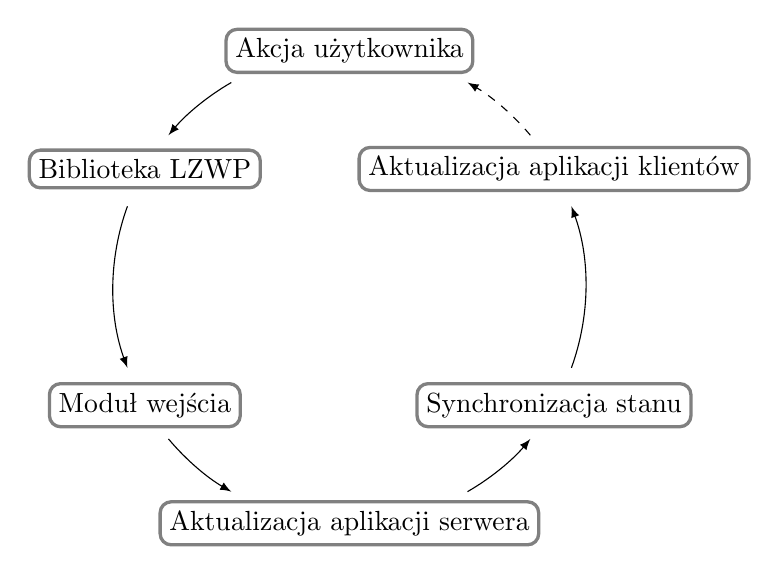
\begin{tikzpicture}[stepstyle/.style={rectangle, 
		rounded corners, draw=gray, very thick,
		text centered, align=center}]
	\def \n {6}
	\def \offset {30}
	\def \radius {3cm}

	\foreach \step [count=\s] in {Akcja użytkownika, Biblioteka LZWP, Moduł wejścia, Aktualizacja aplikacji serwera, Synchronizacja stanu, Aktualizacja aplikacji klientów} {
		\node(\s) [stepstyle] at ({360/\n * (\s) + \offset}:\radius) {\step};
	};
	\foreach \b/\e in {120/140, 160/200, 220/240, 300/320, 340/380} {
		\draw[->, >=latex] ({\b}:\radius)
		arc ({\b}:{\e}:\radius);
	};
		\draw[dashed, ->, >=latex] ({40}:\radius)
		arc ({40}:{60}:\radius);
\end{tikzpicture}
\end{center}
\caption{Diagram kolejności wykonywania modułów przy akcji użytkownika}
\label{fig:diagram-modolow}
\end{figure}



	\section{Zarządzanie pamiecią w aplikacji}
\sectionauthor{Jan Kruczyński}
\label{sec:pamiec}
Ze względu na to, że aplikacja doładowywuje węzły wraz z kolejnymi akcjami użytkownika, gdy przemieszcza się on po grafie lub wskazuje na węzły w przestrzeni, musiał zostać opracowany sposób ich usuwania, by utrzymać płynność działania. Aby to osiągnąć powstał oddzielny kontroler zarządzania pamięcią.

\begin{lstlisting}[caption={Pomocnicze struktury i zmienne kontrolera zarządzania pamięcią}, label=lst:nodePriority]
private List<uint> lowPriorityNodes;%*\label{line:lowPriorityNodes}*)
private List<uint> highPriorityNodes;%*\label{line:highPriorityNodes}*)
public int maxAmountOfNodes;%*\label{line:maxNodes}*)
\end{lstlisting}

Węzły które są załadowane w aplikacji zostały podzielone na dwie kategorie - węzły niskiego priorytetu (\ref{line:lowPriorityNodes}), które są potencjalnymi kandydatami na węzły do usunięcia, oraz wysokiego priorytetu (\ref{line:highPriorityNodes}), których usunąć aktualnie nie można.

Początkowo wszystkie załadowane węzły trafiają do listy niskiego priorytetu. Jeżeli użytkownik dokonuje interakcji z węzłem, to zarówno ten węzeł, jak i wszyscy wyświetlani jego sąsiedzi trafiają do listy wysokiego priorytetu. Jeżeli któryś z tych węzłów znajdował się w liście niskiego priorytetu, jest z niej usuwany i przenoszony na początek listy wysokiego priorytetu.

Funkcjonuje to w taki sposób, aby aplikacja zwalniała w pierwszej kolejności węzły z którymi użytkownik nigdy nie miał interakcji - i dzięki temu nie dostrzegł, że czegoś brakuje. Jednocześnie realizowany jest dodatkowy cel, by ilość wyświetlanych (i przez to przechowywanych w pamięci) węzłów w dowolnej chwili była stała z dokładnością do kilkunastu sztuk.

Kontroler nasłuchuje zdarzenia załadowania węzła przez aplikację. Gdy takie zdarzenie zostanie wykryte, jeżeli liczba wszystkich węzłów, które są wyświetlane w aplikacji, nie przekracza maksymalnej dopuszczonej ilości, nie dzieje się nic. Jeżeli ta liczba zostanie przekroczona, zwalnia kilkanaście węzłów z listy niskiego priorytetu (\ref{line:lowPriorityNodes}).

Gdy lista niskiego priorytetu jest pusta, kontroler przerzuca najstarsze węzły z listy wysokiego priorytetu do listy niskiego priorytetu (są to węzły, z którymi użytkownik prowadził interakcję najdawniej). Gdy użytkownik dokonuje interakcji z węzłem, jest on przerzucany na sam początek listy wysokiego priorytetu.
	\section{Konsola operatora}
\sectionauthor{Mateusz Janicki}
Aplikacja, poza wykorzystaniem flysticków lub klawiatury, może być sterowana za pomocą specjalnej konsoli. Każdorazowe skorzystanie z jaskini wymaga obecności operatora, który uruchamia aplikację w trakcie prezentacji. Będzie on posiadał dostęp do konsoli, a jego zadaniem będzie przenoszenie użytkownika na konkretne węzły przy użyciu wyszukiwarki, a także włączanie zaprogramowanych tras przeglądania grafu. Co więcej, konsola posiada interfejs tworzenia tras umożliwiający szybkie i wygodne tworzenie nowych plików. 

Konsola operatora domyślnie wywoływana jest po naciśnięciu klawisza ''C''. Interfejs posiada dwie zakładki - \textit{Search} oraz \textit{Routes}. Pierwsza jest odpowiedzialna za wyszukiwanie węzłów, na które ma zostać przeniesiony użytkownik, druga służy włączaniu tras. Obydwa elementy posiadają skrypt o nazwie \codeinline{Toggle}, służący odpowiedniemu przełączaniu aktywnych elementów w konsoli. W obu zakładkach znajduje się obiekt przechowujący wyniki wyszukiwania, umieszczane w obiekcie zawierającym komponent  \codeinline{Scroll Rect}. Umożliwia on automatyczne utworzenie paska przewijania, co daje możliwość umieszczenia bardzo dużej ilości elementów.  Dodatkowo w zakładce \textit{Search} znajdują się także obiekt o nazwie  \codeinline{SearchInput} odpowiedzialny za wpisywanie wyszukiwanego węzła, posiadający skrypt  \codeinline{InputField}. Ponadto, nad konsolą znajduje się również informacja o tym, jaki węzeł jest aktualnie wybrany.

\img{\chapterPath/img/console_search.png}{Zrzut ekranu konsoli z otwartą zakładką Search}{console_search}{0.8}
\img{\chapterPath/img/console_routes.png}{Zrzut ekranu konsoli z otwartą zakładką Routes i włączoną trasą}{consoler_routes}{0.8}

Wyszukiwanie węzłów odbywa się na przygotowanym uprzednio pliku, zawierającym posortowane alfabetycznie nazwy artykułów i kategorii oraz ich ID. Przeszukiwanie listy odbywa się za pomocą algorytmu wyszukiwania binarnego. Lista elementów aktualizuje się za każdym wydarzeniem  \codeinline{OnValueChanged} obiektu  \codeinline{SearchInput}. Instancjonowane są kolejne prefaby wyników wyszukiwania, w których zmieniana jest ich pozycja w pionie, nazwa i ikona symbolizująca artykuł lub kategorię. W momencie wybrania węzła wywoływane jest zdarzenie  \codeinline{OnClick}, do którego podpięta jest funkcja  \codeinline{HistoryController} odpowiedzialna za wybranie węzła. Tło wybranego obiektu zmieniane jest na niebiesko.

Lista tras jest pobierana na podstawie aktualnie wybranej wersji Wikipedii. Prefab wyświetlający trasę posiada nazwę, długość trasy oraz przycisk służący jej włączaniu. W celu utworzenia kolejnych elementów listy wykorzystywana jest funkcja  \codeinline{Instantiate()}. W kolejnych instancjach zmieniana jest wysokość obiektu, nazwa przycisku, nazwa trasy oraz długość trasy.  W momencie włączenia trasy wywoływane jest zdarzenie  \codeinline{OnClick}, do którego podpięta jest funkcja  \codeinline{HistoryController} wczytująca trasę o numerze indeksu, którą posiada wciśnięty przycisk. Ponadto tło wybranego obiektu zmieniane jest na niebieski.

	\section{Linia czasu}
\sectionauthor{Mateusz Janicki}
\label{sec:linia-czasu}
Specyfikacja wymagań projektu inżynierskiego zawierała funkcjonalność dotyczącą linii czasu. Wybranie daty miało spowodować wyświetlanie tylko takich węzłów, których data utworzenia była starsza niż wybrana data. Pomogłoby to w przybliżonej wizualizacji, w jak szybki sposób rozrastała się konkretna Wikipedia. Szereg komplikacji spowodował jednak odrzucenie przez nas tej funkcjonalności.

Sterowanie linią czasu miało odbywać się za pomocą drugiego kontrolera. Po wciśnięciu przycisku miał pokazywać się specjalny interfejs ukazujący aktualnie wybraną datę. Można w niej było wybrać, przesuwając joystick w lewo i prawo, miesiąc lub rok, który następnie dałoby się zmieniać przesuwając joystick do góry lub w dół. Zatwierdzenie daty przyciskiem spustu wywoływałoby zmiany w grafie. 

Funkcjonalność nie została zaimplementowana głównie z powodu braku prostej informacji o stworzeniu artykułu w głównie wykorzystywanym przez nas źródle danych, czyli zrzutach baz danych Wikipedii. Istnieją archiwa zawierające kompletną historię edycji artykułów, jednak wielkość tych plików jest nieporównywalnie większa w porównaniu ze zwykłym wykazem stron czy nawet połączeniami pomiędzy stronami. Przetworzenie tych plików tylko po to, aby wydobyć z nich datę pierwszej publikacji strony, jest niewymierna do korzyści wynikających z tej funkcjonalności. 

Innym sposobem wydobycia danych mogłoby być pozyskiwanie tych informacji przy użyciu Wikipedia API. Pomysł ten jednak nie jest wykonalny z powodu ograniczeń, które posiada API. Aby~zdobyć informacje dotyczące każdego artykułu, musielibyśmy wywołać zapytania, których liczba znacznie przewyższa maksymalną dopuszczalną liczbę zapytań dla jednego użytkownika. Przekroczenie tej liczby powoduje zablokowanie adresu IP, z którego pochodziły zapytania i utrudnia dalsze pozyskiwanie danych.

Co więcej, nasza idea linii czasu nie byłaby dokładnym odwzorowaniem stanu Wikipedii w wybranym przez użytkownika czasie. Artykuły i kategorie Wikipedii są bardzo często zmieniane, co implikuje możliwość zmiany połączeń pomiędzy artykułami. Ponadto artykuły i kategorie mogą być także usuwane. Przechowywanie całej historii stron lub stworzenie plików zawierających dokładną historię wszystkich węzłów, jakie kiedykolwiek pojawiły się w Wikipedii, jest niemożliwe na zwykłych komputerach osobistych z powodu zbyt dużej wymaganej przestrzeni na dysku. Nawet jeśli udałoby się je~zapisać, przetwarzanie i wczytywanie takich plików zajęłoby bardzo dużo czasu i spowodowałoby niską responsywność aplikacji. Nasza wersja linii czasu mogłaby być myląca dla nowych użytkowników, którzy mogliby pomyśleć, że przedstawiana jest im dokładna wersja Wikipedii w danym czasie.
	\section{Ostateczny schemat interakcji}
\sectionauthor{Jan Kruczyński}
\label{sec:schemat_interakcji}
Po odrzuceniu funkcjonalności, takich jak widok szczegółowy i linia czasu, możliwa stała się obsługa aplikacji za pomocą tylko jednego kontrolera. Podział na kontroler główny (Rysunek \ref{fig:schemat_kontroler_glowny}) i pomocniczy (Rysunek \ref{fig:schemat_kontroler_pomocniczy}) został odrzucony, a wszystkie interakcje zostały umieszczone na jednym kontrolerze. Ten zabieg znacznie ułatwi użytkownikowi sterowanie aplikacją w jaskini. Nowy schemat sterowania został umieszczony na Rysunku \ref{fig:flystick_new_controls}.

\img{\chapterPath/img/nowy_schemat_kontrolera.png}{Aktualny schemat sterowania kontrolerem}{flystick_new_controls}{0.8}
\end{chapter}




\begin{chapter}{Konfiguracja i uruchamianie}
	\newcommand{\chapterPath}{rozdzialy/5_konfiguracja}
	\label{ch:config}
\end{chapter}

\begin{chapter}{Podsumowanie}
	\newcommand{\chapterPath}{rozdzialy/7_podsumowanie}
\end{chapter}



\input{meta/Bibliografia.tex}

\renewcommand{\baselinestretch}{1.0}\normalsize
\addcontentsline{toc}{chapter}{\listfigurename}
\listoffigures

\addcontentsline{toc}{chapter}{\listtablename}
\listoftables
\renewcommand{\baselinestretch}{1.3}\normalsize

\end{document}
